%%=====================================================================================
%%
%%       Filename:  data-structs-and-algs.tex
%%
%%    Description:  Formal notes of DS and A
%%
%%        Version:  1.0
%%        Created:  02/10/19
%%       Revision:  none
%%
%%         Author:  Josh Felmeden (), nk18044@bristol.ac.uk
%%   Organization:  
%%      Copyright:  Copyright (c) 2019, Josh Felmeden
%%
%%          Notes:  
%%
%%=====================================================================================

% Preamble {{{
\documentclass[11pt,a4paper,titlepage,dvipsnames,cmyk]{scrartcl}
\usepackage[english]{babel}
\typearea{12}
% }}}

% Set indentation and line skip for paragraph {{{
\setlength{\parindent}{0em}
\setlength{\parskip}{1em}
\usepackage[margin=2cm]{geometry}
\addtolength{\textheight}{-1in}
\setlength{\headsep}{.5in}
% }}}

\usepackage{hhline} 
\usepackage{mathtools} 
\usepackage[T1]{fontenc}

% Headers setup {{{
\usepackage{fancyhdr}
\pagestyle{fancy}
\lhead{\rightmark}
\rhead{Data Structures and Algorithms}
\usepackage{hyperref} 
% }}}

% Listings {{{
\usepackage[]{listings,xcolor} 
\lstset
{
    breaklines=true,
    tabsize=3,
    showstringspaces=false
}

\definecolor{lstgrey}{rgb}{0.05,0.05,0.05}
\usepackage{listings}
\makeatletter
\lstset{language=[Visual]Basic,
    backgroundcolor=\color{lstgrey},
    frame=single,
    xleftmargin=0.7cm,
    frame=tlbr, framesep=0.2cm, framerule=0pt,
    basicstyle=\lst@ifdisplaystyle\color{white}\footnotesize\ttfamily\else\color{black}\footnotesize\ttfamily\fi,
    captionpos=b,
    tabsize=2,
    keywordstyle=\color{Magenta}\bfseries,
    identifierstyle=\color{Cyan},
    stringstyle=\color{Yellow},
    commentstyle=\color{Gray}\itshape
}
\makeatother
\renewcommand{\familydefault}{\sfdefault}
% }}}


% Other packages {{{
\usepackage{tkz-graph}
\usepackage{tikz-qtree}
\usepackage{tikz}
\usetikzlibrary{arrows.meta, calc}
\usepackage{amssymb}
\usepackage{graphicx}
\graphicspath{ {./pics/} }
\usepackage{needspace}
\usepackage{tcolorbox}
\usepackage{soul}
\usepackage{babel,dejavu,helvet} 
\usepackage{amsmath} 
\usepackage{booktabs} 
\usepackage{tcolorbox} 
\usepackage[symbol]{footmisc} 
\renewcommand{\thefootnote}{\fnsymbol{footnote}}
\renewcommand{\familydefault}{\sfdefault}
% }}}

% tcolorbox {{{
\newtcolorbox{blue}[3][] {
    colframe = #2!25,
    colback = #2!10,
    #1,
}

\newtcolorbox{titlebox}[3][] {
    colframe = #2!25,
    colback = #2!10,
    coltitle = #2!20!black,
    title = {#3},
    fonttitle=\bfseries
    #1,
}
% }}}

% Title {{{
\title{Data Structures and Algorithms: The formal notes}
\author{Josh Felmeden}
% }}}

\begin{document}

\maketitle
\tableofcontents

\newpage
\section{Greedy algorithms}%
\label{sec:Greedy algorithms}
\subsection{Interval scheduling}%
\label{sub:interval-scheduling}
Let's suppose that you're running a satellite imaging service. Taking a
satellite picture of an area isn't instant and can take some time. It can
also only be done on the day where the satellite's orbit is lined up
correctly. Say you want to request some images to be taken from said
satellite, each of which can only be taken at certain times and you can
only take one picture at a time. How do we satisfy as many requests as
possible?

The requested satellite times that we have to deal with are: 12:00-12:30,
12:05-12:20, 12:15-12:55, 12:20-12:25, 12:38-12:50, and 12:45-13:00.

If we visualise this in a graph, we get: 


\begin{center}
    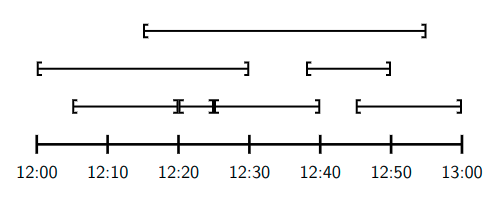
\includegraphics[scale=.5]{graph-satellite.png}
\end{center}

If we take a greedy algorithm approach to assigning these slots, we could
do something like assign the slot that finishes earliest, and then repeat
doing this until we have reached the end. For example, the slot that
finishes fastest is 12:05-12:20, so we assign this. This now removes the
ability for both 12:10-12:30 and 12:15-12:55 to be assigned, so we remove
these. This continues until we end up with something looking like this:


\begin{center}
    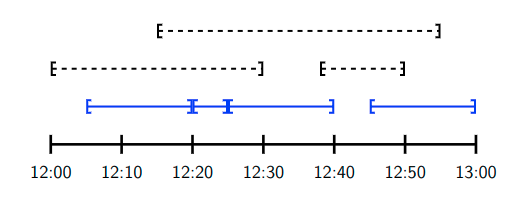
\includegraphics[scale=.5]{graph-assigned}
\end{center}

This means that we satisfy four requests (which is actually the maximum
possible, so well done us).

We can formalise this by saying that a \textbf{request} is a pair of
integers $(s,f)$ with $0 \le s \le f$.

\newpage
The algorithm that we're left with is this:
\begin{lstlisting}
public sub greedySchedule
    sort R
    for each i in {1 ... n} do
        if s_i >= lastf then
            A.append(s_i, f_i)
            lastf = f_i
        end if
    next
end sub
\end{lstlisting}

Now, we need to prove that the output is actually a \textbf{compatible
subset} of R. This is sort of intuitive because the set we added doesn't
break compatibility, since $s \ge$ \lstinline|lastf| and \lstinline|lastf|
is the latest finish time that's already in $A$.

We can formalise this with a loop invariant. At the start of the $i$th
iteration, we see that
\begin{itemize}
    \item $A$ contains a compatible subset $\{(S_1,F_1), \dots,
        (S_t,F_t)\}$ of R.
    \item \lstinline|lastf| = $\max(\{0\} \cup \{F_j : j \le t\})$ 
\end{itemize}

The base case ($i=0$) is immediate because $A = []$. The induction step is
that $A$ was compatible at the start of the iteration, and therefore if we
append a pair $s_i,f_i$ to $A$ then $s \ge $ \lstinline|lastf| $\ge F_j$
for all $f \le t$. This means that $(s_i,f_i)$ is compatible with $A$.


\begin{titlebox}{blue}{Greedy algorithms definition}
Greedy algorithms are actually an informal term and people have different
definitions. The definition that we're going to use is:
\begin{itemize}
    \item They start with a sub-optimal solution.
    \item They look over all the possible improvements and pick the one
        that looks the best at the time.
    \item They never backtrack in `quality'.
\end{itemize}
\end{titlebox}

Greedy algorithms might fail; it's not enough to just do the obvious thing
at each stage. While the algorithms might fail initially, we can use the
knowledge that we gained from the results of the algorithm to design a
more correct one.

\section{Graphs}%
\label{sec:Graphs}

\begin{titlebox}{blue}{Graph Definition}
        A \textbf{graph} is a pair $G = (V,E)$ where $V=V(G)$ is a set of
        \textbf{vertices} $E = E(G)$ is a set of \textbf{edges} contained
        in $\{\{u,v\} : u,v \in V, u \not = \}$
\end{titlebox}

\begin{titlebox}{blue}{Walk Definition}
        A \textbf{walk} in a graph $G = (V, E)$ is a sequence of vertices
        such that $\{v_i, v_{i+1} \in E \text{ for all } i\le k-1$

        We say that the walk is from $v_0$ to $v_k$ and call $k$ the
        length of the walk.
\end{titlebox}


\subsection{Euler walks}%
\label{sub:Euler walks}
An \textbf{Euler walk} is one that contains every edge in $G$
exactly once.

Two graphs might be \textbf{equal}. This is the case when two graphs $G_1
= (V_1, E_1)$ and $G_2 = (V_2, E_2)$ are equal and written $G_1 = G_2$ if
$V_1 = V_2$ and $E_1 = E_2$. This does present some issues, however,
because sometimes graphs look like they should be equal, when they're not
because the edges are labelled differently.

This is where \textbf{isomorphism} comes in. $G_1$ and $G_2$ are
\textbf{isomorphic} if there's a bijection $f: V_1 \rightarrow V_2$ such
that $\{f(u),f(v) \} \in E_2$ if and only if $\{u,v\} \in E_1$.

Intuitively, this means that $G_1 \xrightarrow{\sim} G_2$ if they are the
same graph but the vertices are relabelled.

In a graph $G = (V,E)$, the \textbf{neighbourhood} of a vertex $v$ is the
set of vertices joined to $v$ by an edge. Formally, 
$N_G(v) = \{w \in V : \{v,w\} \in E$. Also, for all sets of vertices
$X \subseteq V = \cup_{v\in X} N_G(v)$

The \textbf{degree} of a vertex $v$ is the \textbf{number} of vertices
joined to $v$. Formally: $d_G(v) = |N_G(v)|$

\textbf{Theorem}: If $G$ has an Euler walk, then either:
\begin{itemize}
    \item Every vertex of $G$ has even degree or
    \item All but two vertices $v_0$ and $v_k$ have even degree, and any
        Euler walk must have $v_0$ and $v_k$ as endpoints.
\end{itemize}

Does every single graph that satisfies both of these conditions have an
Euler walk? No, because the graphs need to be \textbf{connected}.

Within a graph, we also have subgraphs and induced subgraphs. A
\textbf{subgraph} $H = (V_H, E_H)$ of $G$ is a graph with $V_H \subseteq$
and $E_H \subseteq E$. $H$ is an \textbf{induced subgraph} if $V_H
\subseteq V$ and $E_H = \{ e \in E : e \subseteq V_H\}$.

For all vertex sets $X \subseteq V$, the graph is \textbf{induced} by $X$
is:

\begin{center}
    \begin{align*}
        G[X] = (X, \{e \in E: e \subseteq X \})
    \end{align*}
\end{center}

A \textbf{component} $H$ of $G$ is the maximal connected induced subgraph
of $G$, so $H = G[V_H]$ is connected, but $G[V_H \cup \{v\}]$ is
disconnected for all $v \in V \backslash V_H$.

\begin{blue}{blue}
    \textbf{Theorem}: Let $G = (V,E)$ be a \textbf{connected} graph, and
    let $u,v \in V$. Then, $G$ has an Euler walk from $u$ to $v$ if and
    only if either:
    \begin{enumerate}
        \item $u = v$ and every vertex of $G$ has even degree, or
        \item $u \not = v$ and every vertex of $G$ has even degree except
            $u$ and $v$.
    \end{enumerate}
\end{blue}

\section{Sequential Processes}%
\label{sec:sequential-processes}

\section{Fast Fourier Transform}%
\label{sec:fft}

\subsection{Polynomials}%
\label{sub:Polynomials}
A \textbf{degree} $n-1$ polynomial in $x$ can be seen as a function:

\begin{align*}
    A(x) = \sum^{n-1}_{i=0}a_i \cdot x^i
\end{align*}

Any integer that's bigger than the degree of a polynomial is a
\textit{degree bound} of said polynomial. The polynomial $A$ is:

\begin{align*}
    a_0 \cdot x^0 + a_1 \cdot x^1 + a_2 \cdot x^2 \cdots + a_{n-1}x^{n-1}
\end{align*}

The values $a_i$ are the \textit{coefficients}, the degree is $n-1$ and
$n$ is a degree bound. We're able to express any integer as some kind of
polynomial by setting $x$ to some base, say for decimal numbers:

\begin{align*}
    A = \sum^{n-1}_{i=0} a_i \cdot 10^i
\end{align*}

The variable $x$ just allows us to evaluate the polynomial at a point. A
really fast way to evaluate the polynomial is to use \textbf{Horner's
Rule}.

\begin{titlebox}{blue}{Horner's Rule}
Instead of computing all the terms individually, we do:
\begin{align*}
    A(3) = a_0 + 3 \cdot (a_1 + 3\cdot (a_2 + \cdots + 3\cdot (a_{n-1})))
\end{align*}

This method requires $O(n)$ operations. For example, if we consider $A(x) = 2 + 3x + 1.x^2$, we can evaluate this
as:
\begin{align*}
    A(x) = 2 + x(3 + 1.x)
\end{align*}

\end{titlebox}

Once we have our polynomial representations, we might be doing some
arithmetic with them. We're allowed to write polynomials in a
\textit{coefficient representation}. Here, the addition of $C = A + B$
constructs $C$ as the vector:

\begin{align*}
    (a_0 + b_0, a_1 + b_1, a_2 + b_2, \dots, a_{n-1} + b_{n-1})
\end{align*}

$A$ and $B$ should really have the same length, but we're allowed to just
pad the coefficients with zero to make this the case.

\subsubsection{Point value Representation}%
\label{ssub:point-value}
We know that if we're given a polynomial, we can graph it. We can use this
fact to represent a polynomial as a list of its points. For point value
representation, the addition $C = A + B$ constructs $C$ as:

\begin{align*}
    \{x_0, y_0 + z_0),(x_1,y_1 + z_1),(x_2,y_2 + z_2), \dots,
        (x_{n-1},y_{n-1} + z_{n-1})
\end{align*}

where $x_i$ is a point, $y_i = A(x_i) and z_i = B(x_i)$.

It's important to note that the two value representations \textbf{must}
use the same evaluation points. Both of the operations are $O(n)$ in
terms of how long they take.

\subsubsection{Polynomial multiplication}%
\label{ssub:convolution}
Computing a polynomial multiplication (also called \textbf{convolution})
is a little harder than addition. It does, however, become much easier
when we use point value representation:

\begin{align*}
    \{x_0, y_0 \cdot z_0),(x_1,y_1 \cdot z_1),(x_2,y_2 \cdot z_2), \dots,
        (x_{n-1},y_{n-1} \cdot z_{n-1})
\end{align*}

where $x_i$ is a point, $y_i = A(x_i) and z_i = B(x_i)$.

The normal method of calculating multiplication is $O(n^2)$, while using
point value representation only takes $O(n)$. So, is there an easy way to
convert to point value representation? Actually, yes. What we need to do
is to evaluate the polynomial to a point-value representation, multiply
and finally interpolate (the opposite of evaluating) back again.

Long story short, we need to develop two fast algorithms that construct
the coefficients for the point value representation and then
interpolate. So the main steps to multiply the two polynomials $A$ and $B$
(of degree $n$) are:

\begin{enumerate}
    \item \textit{Double degree bound}: Create coefficient representations
        of $A(x)$ and $B(x)$ as degree bound $2n$ polynomials by adding
        $n$ high-order zero coefficients to each.
    \item \textit{Evaluate}: Compute point-value representations of $A(x)$
        and $B(x)$ of length $2n$ through two applications of FFT of order
        $2n$
    \item \textit{Pointwise multiply}: compute a point-value
        representation of $cC(x) = A(x)B(x)$ by multiplying the values
        Pointwise
    \item \textit{Interpolate}: Create a coefficient representation of
        $C(x)$ through a single application of the \textit{inverse} FFT.
\end{enumerate}

The first and third steps are really easy to perform in $O(n)$ time. The
claim is that if we evaluate at the complex roots of unity then we can
perform steps 2 and 4 in $O(n \log n)$ time.

\subsection{Evaluation at roots of unity}%
\label{sub:roots-unity}
First, we need to look at evaluation. We need to evaluate a polynomial of
degree $n$ at $n$ different points. It appears that the complexity of our
method is just going to be $O(n^2)$, but there is a faster way of doing it
than just using Horner's rule. This is when we evaluate the points at
\textit{special} points (namely the \textbf{N-th complex roots of unity}).

\begin{titlebox}{blue}{N-th complex roots of unity}
    \begin{itemize}
        \item The roots of unity are the values $\omega_N = e^{2\pi i j /
            N}$ for $j = 0,1,\dots,N-1$
        \item Say we are evaluating at $N$ pints, we take the N-th complex
            roots of unity $\omega_N$
        \item This means we evaluate the polynomial at the points:
            \begin{align*}
                \omega_N^0,\omega_N^1,\omega_N^2,\dots,\omega_N^{n-1}
            \end{align*}
    \end{itemize}
\end{titlebox}

We want to evaluate a polynomial A at the $n$ roots of unity. Therefore,
we evaluate:
\begin{align*}
    A(x) = \sum_{j=0}^{n-1}a_j \omega_n^{kj}
\end{align*}

for every $k = 0,1,\dots, n-1$

We define the vector of results of these evaluations as:

\begin{align*}
    y_k = A(\omega^k_n)
\end{align*}

This vector $y = (y_0, \dots, y_{n-1})$ is the \textbf{discrete Fourier
Transform} (DFT) of the coefficient vector $a = (a_0, a_1, \dots, a_{n-1})$

\begin{titlebox}{blue}{The Cancellation Lemma}
\begin{align*}
    \omega^{dk}_{dN} = \omega^{k}_{N}
\end{align*}
\end{titlebox}

\begin{titlebox}{blue}{The Halving Lemma}
    If $N > 0$ is even then the squares of the $N$ complex N-th roots of
    unity are the $N/2$ complex $N/2$-th roots of unity

    The proof of this is that we have $(\omega^k_n) ^2 = \omega^k_{n/2}$
    for any nonnegative integer $k$ because of the cancellation lemma.
\end{titlebox}

\subsection{Fast Fourier Transform}%
\label{sub:fft}
The really basic idea of the Fast Fourier transform is that we define two
new polynomials;

\begin{align*}
    A^{[0]}(x) = a_0 + a_2x + \cdots + a_{N-2}x^{N/2 - 1} \\
    A^{[1]}(x) = a_1 + a_3x + \cdots + a_{N-1}x^{N/2 - 1}
\end{align*}

%08/11/19
\section{Dynamic Programming}%
\label{sec:dynamic-programming}
We use \textit{dynamic programming} for finding efficient algorithms for
problems that can be broken down into simpler, overlapping subproblems.
Basically,
\begin{enumerate}
    \item Find a recursive formula for the problem (in terms of answers to
        the subproblems)
    \item Write down a naive recursive algorithm
    \item Speed it up by storing the solutions to the subproblems (\textbf{memoization})
    \item Derive an iterative algorithm by solving the subproblems in good
        order.
\end{enumerate}

\subsection{Weighted interval scheduling}%
\label{sub:weighted-scheduling}
We've seen the scheduling problem before on the course, but this is
different (and as it turns out, harder).

A \textbf{schedule} is a set of compatible intervals. The \textit{weight}
of a schedule is the sum of the weight of the intervals it contains.

We could use a greedy algorithm, but it is really slow and not what we're
looking for. It's not even going to cut it full stop.

\subsubsection*{How is the input provided?}
The intervals are given in an array $A$ of length $n$.

$A[i]$ stores a triple $(s_i, f_i, w_i)$ which defines the $i$th interval.

The intervals are sorted by finish time i.e. $f_i \le f_{i+1}$.=, or the
interval $i$ finishes before the interval $i+1$ finishes.

\subsubsection*{Compatible Intervals}
For all $i$, we let $p(i)$ to be the rightmost interval (in order of
finish time) which finishes before the $i$th interval but doesn't overlap
it.

In the below example, if we take $i = 7$, $p(7) = 3$ because it's the
first interval that doesn't overlap with it (and 3 is the position of the
interval in the array).

\begin{center}
    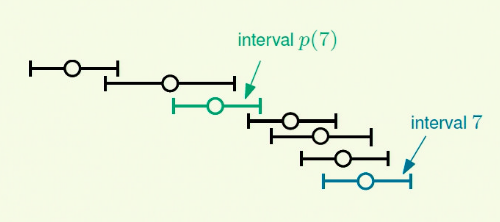
\includegraphics[scale=.5]{weighted-int.png}
\end{center}

$p(4) = 2$, and $p(2) = 0$ because there is no interval that exists.
\textbf{Note} that we index from 1 because otherwise 0 would not make
sense.

\textbf{Claim.} We can precompute all $p(i)$ in $O(n \log n)$ time. For
now, we can assume that this is true, but I will revisit this and prove
why. If you did it naively, it would be $O(n^2)$ time. Obviously it's
something to do with dynamic programming (because that's what this section
is about).

\subsubsection{Finding a solution}%
\label{ssub:solution-dynamic}
Consider some optimal schedule $\mathcal{O}$ for intervals $\{1, 2, 3,
\dots, n\}$ with weight $OPT$. Now, either the $n$th interval is in
schedule $\mathcal{O}$ or it isn't.

Let's look at the case where it is not in $\mathcal{O}$. Schedule
$\mathcal{O}$ is also an optimal schedule for the problem with the input
consisting of the intervals $\{1, 2, 3, \dots, n-1\}$ because $n$ is not in
it. Therefore, in this case, we have $OPT = OPT(n-1)$. (By the way,
$OPT(i)$ is the weight of an optimal schedule for the intervals $\{1,
2, 3, \dots, i\}$).

Now, let's consider the case that it \textbf{is} in $\mathcal{O}$. The
only other intervals that could be in $\mathcal{O}$ are $\{1, \dots,
p(n)\}$. We know that everything larger than $p(n)$ is incompatible with
the $n$th schedule.

\begin{center}
    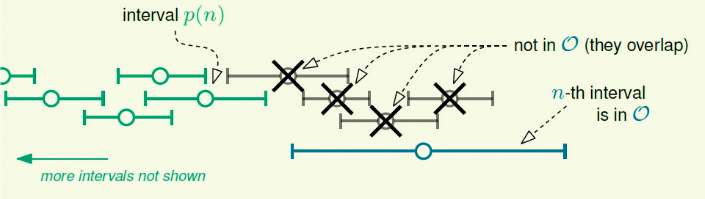
\includegraphics[scale=.5]{weight-n-sched.png}
\end{center}

Schedule $\mathcal{O}$ with interval $n$ removed gives an optimal schedule
for the intervals $\{1, 2, \dots, p(n) \}$ so we now have that $OPT =
OPT(p(n)) + w_n$.

To summarise:
\begin{itemize}
    \item \textbf{Case 1}: The $n$th interval is not in $\mathcal{O}$,
        then $OPT = OPT(n-1)$
    \item \textbf{Case 2}: The $n$th interval is in $\mathcal{O}$, then
        $OPT = OPT(p(n)) + w_n$
\end{itemize}

So, which one do we choose? We choose the bigger one:

\begin{align*}
    OPT = \max (OPT(n-1),OPT(p(n)) + w_n)
\end{align*}

We just now replace all $n$ with $i$ to give us our final recursive
algorithm

\begin{align*}
    OPT = \max (OPT(i-1),OPT(p(i)) + w_i)
\end{align*}

There's no easy way to find these solutions, you just have to kind of look
at the problem for a while and then it will come to you.

\subsubsection{Writing down the recursive algorithm}%
\label{ssub:recursive-written}
Now we have the formula, we get the recursive algorithm:

\begin{lstlisting}
WIS(i)
    If (i=0)
        Return 0
    Return max(WIS(i-1),WIS(p(i)) + wi)
\end{lstlisting}

This algorithm is pretty much exponential given the wrong input. If $T(n)$
is the run time of WIS($n$) using overlapping intervals, then $T(n) >
2T(n-1)$. This is $O(2^{n/2})$.

\subsubsection{Memoization}%
\label{ssub:Memoization}
To solve this, we need to store the solutions to the subproblems.

\begin{lstlisting}
MEMWIS(i)
    If (i=0)
        Return 0
    If WIS[i] undefined
        WIS[i] = max(MEMWIS(i-1),MEMWIS(p(i)) + wi)
    Return WIS[i]
\end{lstlisting}

In this algorithm, we store the solutions to the previously computed
subproblems in an $n$ length array called WIS. The time complexity of
computing MEMWIS($n$) is now $O(n)$. Unfortunately, linear recursion is
still kind of bad.

To compute a value in the array WIS[$i$], we need both WIS[$i-1$] and
WIS[$p[i]$]. Both of these are to the left of WIS[$i$]. Therefore, we
should go through this array from left to right. This is because every
time we compute something, we already have all of the things we need. This
gives us a new algorithm:

\begin{lstlisting}
ITWIS(n)
    If (i=0)
        Return 0
    For i=1 to n
        WIS[i] = max(WIS[i-1], WIS[p(i)] + wi)
\end{lstlisting}

This is an iterative dynamic programming algorithm that runs in $O(n)$
time. The iterative method is better because if we use recursion in $O(n)$
time, we'll probably overload the stack, so this makes the memory
footprint of the algorithm now much smaller. It \textbf{does} however mean
that we need to precompute the $p(i)$ values.

\subsubsection{Computing the p(i) function}%
\label{ssub:Computing the p(i) function}
\textbf{Revised claim.} We can precompute any $p(i)$ in $O(\log n)$ time.
Remember that $s_i$ is the start of interval $i$ and $f_i$ is the finish
time of interval $i$. We want to find the unique value $j = p(i)$ such
that:

\begin{align*}
    f_j < s_i < f_{j+1}
\end{align*}

Because the input is sorted by finish times, we can find $j$ just by using
binary search in $O(\log n)$ time. We can now precompute all $p(i)$ in
$O(\log n)$ time.

% 11/11/19
\section{Dynamic search structures}%
\label{sec:dynamic-search}
A dynamic search structure stores a set of elements. Each element $x$ must
have a unique key: \lstinline|x.key|. The following operations are
supported:

\begin{itemize}
    \item \lstinline|insert(x,k)|: inserts \lstinline|x|  with key \lstinline|k = x.key| 
\end{itemize}
% TODO this

\subsection{Binary search trees}%
\label{sub:bin-search-tree}
Remember that in a binary search tree:
\begin{itemize}
    \item All the nodes in the left subtree have smaller keys
    \item All the nodes in the right subtree have larger keys
\end{itemize}

We perform a \lstinline|find| operation by following a path from the root.

%\begin{tikzpicture}
%    \Tree
%    [.27
%    [.21]]
%\end{tikzpicture}
%% TODO draw a tree

\subsection{2-3-4 Trees}%
\label{sub:2-3-4 Trees}
The idea of this tree is that the nodes can have anywhere between 2 and 4
children (\textit{hence the name}).

\textbf{Perfect balance} means that every path from the root to a leaf has
the same length. Always. Forever.

\begin{itemize}
    \item \textbf{2-node}: 2 children and 1 key
    \item \textbf{3-node}: 3 children and 2 keys
    \item \textbf{4-node}: 4 children and 3 keys
\end{itemize}

Like in a binary search tree, the keys held at a node determine the
contents of its subtrees.

Just like in a binary tree, we have a \lstinline|find| operation. We
perform the operation by following a path from the root. Decisions are
made by inspecting the keys at the current node and following the
appropriate edge.

The time complexity of the \lstinline|find| operation is $O(h)$ again.

\subsubsection{The insert operation}%
\label{ssub:insert}
To perform \lstinline|insert(x,k)|, we need to:
\begin{enumerate}
    \item Search for the key \lstinline|k|  as if we were performing
        \lstinline|find(k)|.
    \item If the leaf is a 2-node, then we insert \lstinline|(x,k)| and
        convert it into a 3-node.
    \item If the leaf is a 3-node, then we insert \lstinline|(x,k)| and
        convert it into a 4-node.
    \item If the leaf is a 4-node, we just make sure it never happens.
\end{enumerate}

\subsubsection{Splitting 4-nodes}%
\label{ssub:split-4-nodes}
We can \lstinline|split| any 4-node into two 2-nodes \textit{if} its
parent isn't a 4-node. For example:

%TODO draw this operation (tikzpicture) Also learn how to use tikz picture
%it seems really useful

We push the extra key up to the parent (which wouldn't work if the parent
is a 4-node). The subtrees haven't changed size, so the path lengths have
not changed due to this \lstinline|split| operation. Therefore, if it was
\textbf{perfectly balanced} before, then it's perfectly balanced after.

\lstinline|splitting| the root increases the height of the tree and
increases the length of all the root-leaf paths by one so it maintains the
\textbf{perfect balance} property. This is the only way that
\lstinline|insert| can affect the lengths of the paths.

Each \lstinline|split| takes $O(1)$ time, so overall \lstinline|insert|
takes $O(\log n)$ time.

\subsubsection{Other operations}%
\label{ssub:other-ops}

\lstinline|Fuse| is an operation that combines two 2-nodes (with the same
parent) into a 4-node (provided the parent isn't a 2-node).

\lstinline|Transferring| keys is possible. If there is a 2-node and a
3-node, we can perform a \lstinline|Transfer| (even if the parent is the
root). No path lengths change from this operation and the time taken is
$O(1)$ time.

\subsubsection{Deleting a node}%
\label{ssub:delete}
To perform \lstinline|Delete(k)| on a \textbf{leaf}, we:
\begin{enumerate}
    \item Search for the key \lstinline|k| using \lstinline|find(k)|. We
        use \lstinline|fuse| and \lstinline|transfer| to convert the
        2-nodes as we go down.
    \item If the leaf is a 3-node, we delete \lstinline|(x,k)|
        %TODO finish this
\end{enumerate}

If we \lstinline|fuse| the root, then the height can decrease by 1. This
is the only time the tree can decrease in height.

If we want to \lstinline|delete| something other than a leaf, we need to:
\begin{enumerate}
    \item Find the \textbf{predecessor} of \lstinline|k| (this is the same
        as \lstinline|find|). This is the element with the largest key
        $k'$ such that $k' < k$
    \item Call \lstinline|delete(k')|. Fortunately, \lstinline|k'| is
        always a leaf
    \item Overwrite \lstinline|k| with another copy of \lstinline|k'|.
\end{enumerate}

\subsection{Summary}%
\label{sub:Summary}
A 2-3-4 tree is a data structure that's based on a tree structure. They are
a little awkward to implement because all nodes don't have the same number
of children. So in practice, we use something called a
\textbf{red-black} tree. It is similar to a binary tree and supports
\lstinline|insert|, \lstinline|find|, \lstinline|delete| functions.

Why do we bother learning these 2-3-4 trees then? Well, they're a little
bit nicer and less complicated to think about and they're basically the
same structure.

%12/11/19
\section{Making shortcuts}%
\label{sec:shortcuts}
What happens if we add some shortcuts to a set of nodes. Because in the
real world it's possible to take shortcuts in terms of a train line or
something similar.

We might attach a second linked list containing only some of the keys. How
do we now perform \lstinline|find(k)| in this linked list?

To perform \lstinline|find| we start in the top list and go right until
we come to a key $k' > k$. Then, we move down to the bottom list and go
right until we find $k$. Imagine that we decide to place $m$ keys in the
top list, and the bottom list contains $n$ keys (this will always be true
since the bottom list has all of the keys). Where should we put the $m$
keys to minimise the \textit{worst} case (for a find operation)?

If we spread out the $m$ keys evenly, we get the biggest overall
improvement. If we do an uneven spread, some of the keys will be found
really fast, but there will be some poor cases, and since we're trying to
minimise the worst case, we want to make sure all cases are catered for.
Now, the worst case time for a \lstinline|find| operation becomes $O(m +
n/m)$.

By setting $m = \sqrt{n}$, we get the \textbf{worst case} time for a
\lstinline|find|  operation to be $O(\sqrt{n})$.

\subsection{More levels}%
\label{sub:levels}
We've looked at having 2 lists, but what if we have more than that? The
more levels we introduce, the better it gets. Each \textit{level} will
contain \textbf{half} of the keys (called rounding up) from the level
below. They are chosen to be spread as evenly as possible.

The bottom level still contains every key, and every level contains the
leftmost and rightmost keys.

since each level has half of the keys from the below level, there are
$O(\log n)$ levels (kinda like a tree). 

% Write the notes from this lecture my laptop died TODO

% lecture from 15/11/19
\section{Line segments}%
\label{sec:line-segments}
Consider $n$ line segments. Find all of the intersections. How do we go
about this?

The simplest algorithm is to test every pair of line segments.

Let $s_i$ denote the $i$-th line intersection:
\begin{lstlisting}
for i = 1,2, ..., n
    for j = 1,2, ...,n
        if (s[i] intersects s[j]) and (i != j)
            output (i,j)
\end{lstlisting}

Given two line segments $s_i$ and $s_j$, described by their end point
coordinates, we can decide whether (and also where) they intersect in
$O(1)$ time. This can be proved because any computation on two objects
with $O(1)$ (constant) space descriptions take $O(1)$ time. It doesn't
tell you how to do it, but just know that this is true.

The algorithm above, however, runs in $O(n^2)$ time (because checking each
pair of lines takes $O(1)$ time).

If there are $n$ line segments we could have a maximum of $(n/2)^2$
intersections. If we want to output all of the intersections, then we
can't expect to do better than $O(n^2)$ in the worst case simply because
the time complexity of printing the output.

\subsection{Output sensitive algorithms}%
\label{sub:ouput-sensitive}
Up to this point in the course, we've only looked at how the actual
input affects the runtime. With this algorithm, however, we also need
to consider the size of the output.

Eventually, we'll work up to an algorithm with runtime $O(n \log n + k
\log n)$. When $K$ is really big, then this algorithm is actually worse
than the naive algorithm with $O(n^2 \log n)$. But, when $k$ is small, the
algorithm is much better with $O(n \log n)$.  

\newpage
\subsection{Simplifying restrictions}%
\label{sub:simplifying-restriction}
To make things a bit easier, we are not allowing:
\begin{itemize}
    \item Horizontal line segments
    \item Two end points with the same %y% coordinates
    \item Three or more line segments that intersect at the same point
    \item Overlapping line segments
\end{itemize}

\subsection{First observation}%
\label{sub:first-ob}
The \textbf{$y$-span} of $s_i$ is the range of the $y$ axis that $s_i$
takes. From this definition, if $s_i$ and $s_j$ don't have overlapping
$y$-spans, they don't intersect. This method suggests an overall approach
called \textit{line sweeping}. We sweep a horizontal line through the
plane from top to bottom and find intersections as we go.

When we see that there are two lines in the same $y$-span that are also
next to each other, we say that the two lines are \textit{adjacent}
\textbf{at this $y$-coordinate}. Some pair of lines that are adjacent at
some $y$ coordinate may not be adjacent at another because another line
might come between them.

\textbf{Note!} Two line segments that are \textit{never} adjacent
\textbf{cannot intersect}. Intuitively, if they are never actually next to
each other, they cannot cross.

\subsubsection{Event points}%
\label{ssub:event-points}
The \textbf{event points} are the `interesting positions' of a line, which
we define as the end points of the line and the intersection points. We
have to detect the intersection points on the fly \textbf{before} we get
to them.

The total number of event points is $O(n + k)$ where $n$ is the number of
endpoints and $k$ is the number of intersections.

\subsubsection{Status of the sweep line}%
\label{ssub:status-sweep-line}
The status of the sweep line is the set of line segments that currently
intersect the sweep line. We order this from \textit{left to right} by
where they intersect.

The status of the sweep line can only change at event points.

We will store the status of the sweep line in a data structure. This allows
efficient updates.

\subsubsection{Updating the sweep line}%
\label{ssub:update-sweep-line}
Every time the sweep line moves to the next event point, we update the
status data structure. If the event point is the \textit{top of a line
segment}, we insert it into the status data structure at the appropriate
place (using the insert function).

Then, we check whether the segment will intersect either of the adjacent
segments.

If the event point is the \textit{bottom of a line segment} then we delete
it from the status data structure.

Finally, if the event point is an \textit{intersection point}, we
\textbf{swap} the two line segments in the data structure.

% Lecture from 25/11/19
\section{Shortest Path Revisited}%
\label{sec:shortest-path-revisited}
We've already looked at the shortest path thing, but now, we're going to
do it with negative weights. Bellman-Ford's algorithm solves the
\textbf{single source shortest paths} problem (in a weighted directed
graph).

It finds the shortest path from a given \textit{source} vertex to every
other vertex. The weights are allowed to be both positive and negative,
and the graph is stored as an \textbf{adjacency list}.

\subsection{Negative weight cycles}%
\label{sub:negative-cycles}
If some of the edges in the graph have negative weights, the idea of a
shortest path might not make sense:

%TODO draw a negative cycle using tikz

A negative weight cycle is a path from a vertex $v$ back to $v$ such that
the sum of the edge weights is negative. If there is a path from $s$ to
$t$, which includes a negative weight cycle, there is no shortest path
from $s$ to $t$.

Firstly, we are going to discuss a simpler version of the Bellman-Ford
algorithm, that assumes there are \textbf{no such cycles}.

The algorithm repeatedly asks, for every edge $(u,v)$ ``can I find a
shorter route to $v$ if I go via $u$?". Here is the algorithm:

\begin{lstlisting}
sub MostOfBellman-Ford
    for all v, set dist(v) = infinity
    set dist(s) = 0
    for i = 1 to |V|
        for each edge (u,v) in E
            if dist(v) > dist(u) + weight(u,v) then
                dist(v) = dist(u) + weight(u,v)
            end if
        next
    next
end sub 
\end{lstlisting}

This algorithm runs $|V|$ iterations. In each iteration, we relax
\textbf{every} edge $(u,v)$.

Now, consider the algorithm where in each algorithm you relax every edge
(instead of only one). After enough iterations, we get all edges to be the
shortest path. But, how many iterations is enough? Well, we need to do one
iteration for each node in the path we want to find the shortest path of.

Due to the fact that we have no negative weight cycles, deleting a cycle
from a path \textbf{cannot} increase its length. Therefore, there is a
shortest path between two nodes containing no cycles.  Therefore, we have
proved that `enough' cycles is $|V|$.

Of course, if there is no path between the two nodes, then at termination,
\lstinline|dist(v) = infinity|. If there is a shortest path between two
nodes, then it contains at most $|V|$ edges (assuming there are no
negative weight cycles).

So, what's the rest of the algorithm?

\subsection{The rest of the algorithm}%
\label{sub:rest-of-alg}

\begin{lstlisting}
sub bellman-ford
    for all v, set dist(v) = infinity
    set dist(s) = 0
    for i = 1 to |V|
        for each edge (u,v) in E
            if dist(v) > dist(u) + weight(u,v) then
                dist(v) = dist(u) + weight(u,v)
            end if
        next
    next

    for each edge (u,v) in E
        if dist(v) > dist(u) + weight(u,v)
            print("negative weight cycle found")
        end if
    next
end sub
\end{lstlisting}

The final check outputs a message if there is a negative weight cycle, and
it does this by checking if there is a path that is shorter than the
shortest path (that is a contradiction) and therefore there must be a
negative weight cycle.

\newpage
% Lecture 26/11/19 (last raphael clifford lecture :( )
\subsection{All-pairs Shortest Paths}%
\label{sub:all-pairs-shortest}
In previous lectures, we have focused on the single source graphs, But,
what if we want to find the shortest paths from every vertex to every other
vertex?

\begin{itemize}
    \item If the graph has \textbf{non-negative edge weights}, then we can
        just run Dijkstra's algorithm $|V|$ times. ($O(|V||E|\log|V|)$
        time).
    \item If the graph has both \textbf{positive and negative edge
        weights}, we can repeatedly run Bellman-Ford's algorithm.
        ($O(|V|^2|E|)$ time)
\end{itemize}

The output contains the length of the shortest path between every pair of
vertices, so there are $|V| \cdot (|V|-1)$, therefore we can't expect to
do better than $O(|V|^2)$, based on pairs alone.

Now, imagine that $|E| \approx \frac{|V|^2}{4}$ (basically ,each vertex
has an edge to about half of the other vertices). This is quite a dense
graph. If $V$ was 10000, then this becomes just too big.

If the graph is really sparse ($|E| \approx 5|V|$), (basically each vertex
has an edge to about 5 other vertices). 

\subsubsection{Johnson's algorithm}%
\label{ssub:johnson's-algorithm}
We've already seen one algorithm for all-pairs shortest paths that takes
$O(|V||E|\log|V|)$ time.If the graph had non-negative weights, we can just
repeatedly apply Dijkstra's algorithm. However, we are interested in graphs
that have both positive and negative edge weights. The approach employed
by Johnson's algorithm is to reweight the edges so that the resulting
graph has non-negative edge weights, and \textit{then} repeatedly runs
Dijkstra's algorithm. For example;

%GRAPH EXAMPLE (ALSO TODO)
\begin{center}
\begin{tikzpicture}
    \begin{scope}[every node/.style={circle,thick,draw}]
        \node (A) at (0,2) {A};
        \node (B) at (2,0) {B};
        \node (C) at (4,2) {C};
        \node (D) at (2,4) {D};
    \end{scope}

    \begin{scope}[>={Stealth[black]},
        every node/.style={fill=white,circle},
        every edge/.style={draw=black,very thick}]
        \path [->] (A) edge node {$0$} (B);
        \path [->] (C) edge node {$-2$} (A);
    \end{scope}
\end{tikzpicture}
\end{center}

%TODO some bits here (I was messing around with some graph shit)

\subsection{Reweighted paths}%
\label{sub:reweighted-path}
Let the function $h$ give a value $h(v)$ for each vertex $v \in V$ change
the weight of every edge $(u,v)$ to be:
\begin{align*}
    \text{weight}'(u,v) = \text{ weight}(u,v) + h(u) - h(v)
\end{align*}

\textbf{Lemma}: Any path is a shortest path in the original graph if and
only if it is a shortest path in the reweighted graph. 

In summary, to reweight the graph, we let the function $h$ give a value
$h(v)$ for each vertex $v\in V$. Then, we change the weight of every edge
$(u,v)$ to be $\text{weight}'(u,v) = \text{ weight}(u,v) + h(u) - h(v)$.

\textbf{Lemma}: Any path is a shortest path in the original graph if and
only if it is a shortest path in the reweighted graph.

\textbf{Fact}: If $\ell$ is the length of a path from $u$ to $v$ %** TODO

\subsection{Choosing h}%
\label{sub:Choosing-h}
We first add one additional vertex called $s$ to the original graph. We
also add an edge $(s,v)$ from $s$ to each other vertex $v \in V$ (each of
the edges has weight 0). For each $v$, let $\delta(s,v)$ denote the length
of the shortest path from $s$ to $v$. We then define $h(v)$ to equal
$\delta(s,v)$.

Consider any edge $(u,v) \in E$. The key observation is that $\delta(s,v)
\le \delta(s,u) + \text{ weight}(u,v)$. Rearranging this, we end up with
$\text{weight}'(u,v) = \text{ weight} (u,v) + h(u) - h(v)$.

\subsection{Johnson's actual algorithm}%
\label{sub:real-johnson}
We can now piece together Johnson's algorithm which operates as follows:
\begin{enumerate}
    \item Add one additional vertex called $s$ to the original graph
    \item For each vertex, add an edge $(s,v)$ with weight 0
    \item Run the Bellman-Ford algorithm with source $s$. (This calculates
        the shortest path lengths $\delta(s,v)$) for all $v$.
    \item Reweight each edge $(u,v) \in E$ so that 
        \begin{align*}
            \text{weight}'(u,v) = \text{ weight}(u,v) + h(u) - h(v)
        \end{align*}
    \item For each vertex $u$, run Dijkstra's algorithm with source $s =
        u$.
    \item For each pair of vertices $u,v$ compute
        \begin{align*}
            \delta(u,v) = \delta'(u,v) + h(v) - h(u)
        \end{align*}
\end{enumerate}

Therefore, the overall time complexity is $O(|V||E|\log|V|)$, which is
actually the same time period as Dijkstra's algorithm.

\section{Linear Programming}%
\label{sec:linear-programming}
Linear programming is one of the most useful techniques for solving
optimisation problems. It's used in loads of things, so let's look at an
example.

Say (God forbid) we decided we liked Warhammer. Now, let $N$ be the number
of `noise marines' Games Workshop produces in a day and $D$ be the number
of `Doomwheels'. The numbers are as follows:

\begin{itemize}
    \item Games Workshop makes a profit of £$4$ per noise marine and
        £$10$ per doomwheel. They therefore want to \textbf{maximise} $4N
        + 10D$. 
    \item Their plastic plant can turn out 5kg of finished parts every
        day. One noise marine has 5g plastic, and a doomwheel contains
        100g. Therefore, $5N + 100D \le 5000$
    \item Similarly, their metal plant is able to turn out 4kg of finished
        parts every day. One noise marine has 60g of metal, while a
        doomwheel has 10g, so they also require that $60N + 10D \le 4000$.
    \item They believe that they can sell up to 100 noise marines and 50
        doomwheels per day, but no more so they require that $N \le 100$
        and $D \le 50$.
    \item Games workshop obviously can't produce a negative amount of
        either figure, so $N, D \ge 0$
\end{itemize}

To formalise, the problem we're looking at is:
\begin{align*}
    4N + 10D &\rightarrow \max, \text{ subject to } \\
    5N + 100D &\le 5000;\\
    50N + 10D &\le 4000;\\
    N &\le 100;\\
    D &\le 50;\\
    N, d &\ge 0
\end{align*}

We can actually convert this into a matrix:
\begin{align*}
    4N + 10D &\rightarrow \max, \text{ subject to } \\
\begin{pmatrix}
    5 & 100 \\
    60 & 10 \\
    1 & 0 \\
    0 & 1
\end{pmatrix}
\begin{pmatrix}
    N \\
    D
\end{pmatrix}
&\le
\begin{pmatrix}
    5000 \\
    4000 \\
    100 \\
    50
\end{pmatrix}
\\
N, D &\ge 0
\end{align*}

We say that $\vec x \le \vec y$ iff $\vec x_i \le \vec y_i$ for all $i$,
and the same for $\vec x \ge \vec y$.

For example, $(2,0,1) \ge (0,0,0)$ but $(2,0,1) \not \ge (0,1,0)$. Despite
this, we also have $(2,0,1) \not \le (0,1,0)$ because they are
incomparable.

What if we were to have a linear \textbf{objective function}
$f:\mathbb{R}^n \rightarrow \mathbb{R}$, an  $m \times n$ matrix $A$ and
an $m$-dimensional vector $\vec b \in \mathbb{R}^m$? The desired output is
a vector $\vec x \in \mathbb{R}^n$ maximising $f(\vec x)$ subject to $A
\vec x \le \vec b$ and $\vec x \ge \vec 0$.

We say that a $\vec x in \mathbb{R}^n$ is a \textbf{feasible} solution to
a linear program if $\vec x \ge 0$ and $A \vec x \le b$, and it's an
\textbf{optimal} solution if $f(\vec y) \le f(\vec x)$ for all feasible $y
\in \mathbb{R}^n$.

Sometimes, there are no optimal solutions, and this could be for two
reasons:

\begin{enumerate}
    \item Sometimes, the constraints are really tight, so they rule out
        \textit{any} feasible solutions at all. This means that $x
        \rightarrow \max$ subject up to $x \le -1$ and $x \ge 0$.
    \item Sometimes, the constraints are so loose that there are feasible
        solutions with $f(\vec x)$ that is arbitrarily large. This means
        $x \rightarrow \max$ subject to $x \ge 0$.
\end{enumerate}

These are the only two things that can go wrong. All you need to know is
that any bounded linear program that has at least a single feasible
solution has an optimal solution.

The statements that we've made seem a little restrictive. What if we look
into minimisation problems, or equality constraints or allowing variables
to be negative? Well, we can implement these in the framework we've
defined, in something known as \textbf{standard form}.

I don't mean that classic scientific standard form. Let's take an example
and turn this linear program (LP) into standard form.
\begin{align*}
    4x - 5y + z &\rightarrow \min \text{ subject to } \\
    x + y + z &= 5; \\
    x + 2y &\ge 2; \\
    x, z &\ge 0
\end{align*}

In the example of the \textbf{minimisation problem}, we want $f(\vec x)$
to be as small as possible if and only if $-f(\vec x)$ is as large as
possible. Therefore, $4x-5y+z \rightarrow \min$ is equivalent to $-4x+5y-z
\rightarrow \max$.

Let's apply these changes:
\begin{align*}
    {\color{blue} \mathbf{-4x+5y-z}} &{\color{blue}\rightarrow \max \text{ subject to }} \\
    x + y + z &= 5; \\
    x + 2y &\ge 2; \\
    x, z &\ge 0
\end{align*}

Now we look at the constraints. $\Sigma_i a_i x_i = b_i$ if and only if
$\Sigma_i a_i x_i \ge b_i$ \textbf{and} $\Sigma_i a_i x_i \le b_i$.
Knowing this, $x + y + z = 5$ is equivalent to $x + y + z \le 5$
\textbf{and} $x + y + z \ge 5$.

 
Similarly, $\Sigma_i a_i x_i \ge b_i$ if and only if
$-\Sigma_i a_i x_i \le b_i$ \textbf{and} $\Sigma_i a_i x_i \le b_i$.
So, $x + 2y \ge 2$ is the same as $- x - 2y \le -2$ and also $x + y + z
\ge 5$ (from the previous constraint) is the same as $-x -y -z \le -5$

This leaves us with
\begin{align*}
    -4x+5y-z &\rightarrow \max \text{ subject to } \\
    {\color{blue}x + y + z} &{\color{blue}\le 5;} \\
    {\color{blue}x - y - z} &{\color{blue}\le -5;} \\
    {\color{blue}x - 2y} &{\color{blue}\le -5;} \\
    x, z &\ge 0
\end{align*}

Now, we can remove the non-negativity. This means that if $y$ doesn't have
to be non-negative, we can replace it with $y_1 - y_2$ where $y_1, y_2 \ge
0$. We think of $y_1$ as the positive part and $y_2$ as the negative part.
There will be a feasible solution with both $y_1, y_2 > 0$, but this
doesn't actually matter. Any optimal solution of the old problem is an
optimal solution of the new one and vice versa.

Now we get:
\begin{align*}
    -4x+5{\color{blue}(y_1 - y_2)}-z &\rightarrow \max \text{ subject to } \\
    {\color{blue}x + {\color{blue}(y_1 - y_2)} + z} &{\color{blue}\le 5;} \\
    {\color{blue}- x - {\color{blue}(y_1 - y_2)} - z} &{\color{blue}\le -5;} \\
    {\color{blue} -x - 2{\color{blue}(y_1 - y_2)}} &{\color{blue}\le -2;} \\
    x,{\color{blue}(y_1, y_2)},z &\ge 0
\end{align*}

And finally, we get the matrix:
\begin{align*}
    \begin{pmatrix}
        -4 & 5 & -5 & -1 \\
        1 & 1 & -1 & 1 \\
        -1 & -1 & 1 & -1 \\
        -1 & -2 & 2 & 0
    \end{pmatrix}
    \begin{pmatrix}
        x \\
        y_1 \\
        y_2 \\
        z
    \end{pmatrix}
    &\le
    \begin{pmatrix}
        5 \\
        -5 \\
        -2
    \end{pmatrix} \\
    x,y_1,y_2,z &\ge 0
\end{align*}

The problem is now in standard form and the techniques are completely
general. What we've done is reduced the problem of having to solve a
linear program which might have any sort of things to that of solving a
linear program in standard form. This makes it so much easier to find an
algorithm.

We are also able to plot the linear program geometrically by plotting all
of the $\le$s as a graph and then taking the areas under them. Because we
can do this, we also must note that there will be an optimal solution at a
corner.

\subsection{Simplex algorithm}%
\label{sub:simplex-alg}
The $n$-variable constraints of an LP describe a feasible polytope in
$\mathbb{R}^n$. If the linear program does have an optimal solution (so
it's bounded and the feasible polytope is non-empty), then it will have
one at the vertex of the polytope (the polytope being the shape made when
we pot the graphs).

The simplex algorithm can be boiled down to a \textbf{greedy search} for a
vertex of the feasible polytope that maximises the objective function.

If we start at an arbitrary vertex, we look at all the neighbouring
vertices and move the whichever one makes the objective function largest.
If none of the vertices match this, then we just return the current
vertex. The problem is that there are often $\Omega(2^n)$ vertices such as
with a hypercube.

\subsubsection{Runtime of the Simplex Algorithm}%
\label{ssub:runtime-simplex}
Intuitively, it feels like there should always be a short path from any
vertex to an optimal solution, but unfortunately the simplex algorithm
doesn't have to find the shortest path. There exists a shape where the
greedy algorithm needed to visit every single vertex.

In practice, it only needs $\Theta(n)$ steps. To prove this is actually an
open problem in theoretical computer science. There are also
\textit{interior point algorithms} which have a polynomial worst-case
run-time, but they work less well in practice.

\subsection{Approximation Algorithms}%
\label{sub:aprox-algorithms}
A vertex cover in a graph $G=(V,E)$ is a set $X \subseteq V$ such that
every edge in $E$ has at least a single vertex in $X$. =

For example:

\begin{figure}[htpb]
\begin{center}
    \begin{tikzpicture}[%
    cloud/.style={
      draw=red,
      thick,
      ellipse,
      fill=red!20,
      minimum height=1em
    }]
    \GraphInit[vstyle=Classic]
    \SetGraphUnit{1.5}
    \tikzset{VertexStyle/.style = {shape = circle,fill = black,minimum size = 7,inner sep=0}}
    \node[VertexStyle] at (1,3) (1) {};
    \node[VertexStyle] at (2,3) (2) {};
    \node[VertexStyle] at (0,2) (3) {};
    \node[VertexStyle] at (3,2) (4) {};
    \node[VertexStyle] at (0,1) (5) {};
    \node[VertexStyle] at (3,1) (6) {};
    \node[VertexStyle] at (1,0) (7) {};
    \node[VertexStyle] at (2,0) (8) {};

    \path[draw,thick]
        (1) edge node {} (2)
        (1) edge node {} (3)
        (2) edge node {} (4)
        (2) edge node {} (5)
        (3) edge node {} (5)
        (3) edge node {} (4)
        (4) edge node {} (6)
        (5) edge node {} (6)
        (5) edge node {} (2)
        (5) edge node {} (7)
        (7) edge node {} (8)
        (7) edge node {} (3)
        (8) edge node {} (2)
        ;

    \draw[thick,red]     ($(2.north west)+(-0.1,0.1)$) rectangle
        ($(2.south east)+(0.1,-0.1)$);
    \draw[thick,red]     ($(3.north west)+(-0.1,0.1)$) rectangle
        ($(3.south east)+(0.1,-0.1)$);
    \draw[thick,red]     ($(6.north west)+(-0.1,0.1)$) rectangle
        ($(6.south east)+(0.1,-0.1)$);
    \draw[thick,red]     ($(7.north west)+(-0.1,0.1)$) rectangle
        ($(7.south east)+(0.1,-0.1)$);
\end{tikzpicture}
\quad\quad\quad
\begin{tikzpicture}[%
    cloud/.style={
      draw=red,
      thick,
      ellipse,
      fill=red!20,
      minimum height=1em
    }]
    \GraphInit[vstyle=Classic]
    \SetGraphUnit{1.5}
    \tikzset{VertexStyle/.style = {shape = circle,fill = black,minimum size = 7,inner sep=0}}
    \node[VertexStyle] at (1,3) (1) {};
    \node[VertexStyle] at (2,3) (2) {};
    \node[VertexStyle] at (0,2) (3) {};
    \node[VertexStyle] at (3,2) (4) {};
    \node[VertexStyle] at (0,1) (5) {};
    \node[VertexStyle] at (3,1) (6) {};
    \node[VertexStyle] at (1,0) (7) {};
    \node[VertexStyle] at (2,0) (8) {};

    \path[draw,thick]
        (1) edge node {} (2)
        (1) edge node {} (3)
        (2) edge node {} (4)
        (2) edge node {} (5)
        (3) edge node {} (5)
        (3) edge node {} (4)
        (4) edge node {} (6)
        (5) edge node {} (6)
        (5) edge node {} (2)
        (5) edge node {} (7)
        (7) edge node {} (8)
        (8) edge node {} (2)
        ;
    \path[draw,thick,dashed,green]
        (7) edge node {} (3)
        ;

    \draw[thick,red]     ($(1.north west)+(-0.1,0.1)$) rectangle
        ($(1.south east)+(0.1,-0.1)$);
    \draw[thick,red]     ($(4.north west)+(-0.1,0.1)$) rectangle
        ($(4.south east)+(0.1,-0.1)$);
    \draw[thick,red]     ($(5.north west)+(-0.1,0.1)$) rectangle
        ($(5.south east)+(0.1,-0.1)$);
    \draw[thick,red]     ($(8.north west)+(-0.1,0.1)$) rectangle
        ($(8.south east)+(0.1,-0.1)$);
\end{tikzpicture}
\end{center}
\end{figure}

The left graph is an example of a valid vertex cover, while the right is
\textbf{not} a valid vertex cover. We want to find the smallest possible
vertex cover of $G$.

We can express finding a minimum vertex cover as solving a linear program,
where the solutions are integers. This is an \textbf{integer linear
program}.

Given some graph $G = (V,E)$, we assign a variable $x_v \in \{0,1\}$ to
each vertex $v$. We interpret $x_v = 1$ as ``$x_v$  is in the cover'', and
$x_v =0$ as ``$x_v$ is not in the cover". We can then formulate the
problem as:

\begin{alignat*}{2}
    \Sigma_i x_i &\rightarrow \min \text{ subject to } &\text{Minimise }
    |X| \text{ subject to} \\
    x_u + x_v &\ge 1 \text{ for all } \{u,v\} \in E; \quad \quad \quad &u\in X \text{ or }
    v\in X \text{ (or both)} \\
              &\text{} &\text{for all } \{u,v\} \in E \\
    x_v &\le 1 \text{ for all } v \in V; &\text{} \\
    x_v &\ge 0 \text{ for all } v \in V; &[\text{Ensures } x_v \in \{0,1\}
    \text{ for all } v] \\
    x_v &\in \mathbb{N} \text{ for all } v \in V 
\end{alignat*}

In this example:
\begin{center}
    \begin{tikzpicture}
        \tikzset{VertexStyle/.style = {shape = circle,fill = black,minimum size = 7,inner sep=0}}
    \node[VertexStyle] [label={[label distance=0cm]90:1}] at (1,3) (1) {1};
    \node[VertexStyle] [label={[label distance=0cm]90:8}] at (2,3) (2) {8};
    \node[VertexStyle] [label={[label distance=0cm]180:2}] at (0,2) (3) {2};
    \node[VertexStyle] [label={[label distance=0cm]0:7}] at (3,2) (4) {7};
    \node[VertexStyle] [label={[label distance=0cm]180:3}] at (0,1) (5) {3};
    \node[VertexStyle] [label={[label distance=0cm]0:6}] at (3,1) (6) {6};
    \node[VertexStyle] [label={[label distance=0cm]-90:4}] at (1,0) (7) {4};
    \node[VertexStyle] [label={[label distance=0cm]-90:5}] at (2,0) (8) {5};

    \path[draw,thick]
        (1) edge node {} (2)
        (1) edge node {} (3)
        (2) edge node {} (4)
        (2) edge node {} (5)
        (3) edge node {} (5)
        (3) edge node {} (4)
        (4) edge node {} (6)
        (5) edge node {} (6)
        (5) edge node {} (2)
        (5) edge node {} (7)
        (7) edge node {} (8)
        (8) edge node {} (2)
        ;
    \path[draw,thick,dashed,green]
        (7) edge node {} (3)
        ;

    \draw[thick,red]     ($(1.north west)+(-0.1,0.1)$) rectangle
        ($(1.south east)+(0.1,-0.1)$);
    \draw[thick,red]     ($(4.north west)+(-0.1,0.1)$) rectangle
        ($(4.south east)+(0.1,-0.1)$);
    \draw[thick,red]     ($(5.north west)+(-0.1,0.1)$) rectangle
        ($(5.south east)+(0.1,-0.1)$);
    \draw[thick,red]     ($(8.north west)+(-0.1,0.1)$) rectangle
        ($(8.south east)+(0.1,-0.1)$);
\end{tikzpicture}
\end{center}

$X = \{1,3,5,7\}$ is \textbf{not} a vertex cover. Here we have $x_1 = x_2
= x+5 = x+7 = 1$ and $x_0 = x_2 = x_4 = x_6 = 0$. The uncovered edge
$\{2,4\}$ corresponds to the constraint $x_2 + x_4 \ge 1$.

So that's it, yeah? We can just solve the ILP? Nah, it's generally
impossible to solve ILP's efficiently. It's also impossible to find a
minimum vertex cover efficiently unfortunately.

We \textit{can} solve LPs though. If we \textbf{relax} our ILP to allow
non-integer solutions, therefore turning it into an LP, we might be able
to solve it. That leaves us with:
\begin{align*}
    \Sigma_i x_i &\rightarrow \min \text{ subject to } \\
    x_u + x_v &\ge 1 \text{ for all } \{u,v\} \in E; \quad \quad \quad \\
    x_v &\le 1 \text{ for all } v \in V; \\
    x_v &\ge 0 \text{ for all } v \in V; \\
    x_v &\in \mathbb{N} \text{ for all } v \in V
\end{align*}

Then, we take our vertex cover $X$ to be $\{v \in V : x_v \ge 1/2\}$,
basically rounding up to recover a feasible solution for the ILP. It's not
that hard to show that if a minimum vertex cover has size $k$, then $X$ is
indeed a vertex cover and $k \le |X| \le 2k$. This is an approximate
solution to a really tough problem.

\section{Flow Algorithms}%
\label{sec:flow-algorithms}
\subsection{Flow networks}%
\label{sub:flow-networks}
\textbf{Flow networks} are where something is travelling from place to
place inside a graph. Examples might include stuff like water networks or
power networks and so on.

More generally, a flow network $(G,c,s,t)$ consists of a directed graph $G
= (V,E)$. A capacity function $c : E \rightarrow \mathbb{N}$, a
\textbf{source vertex} $s \in V$ with $N^- (s) = \empty$ and a
\textbf{sink} vertex $t \in V$ with $N^+(t) = \empty$.

A \textbf{flow} in $(G,c,s,t)$ is a function $f:E \rightarrow \mathbb{R}$
with:
\begin{itemize}
    \item No edge has more flow than the capacity, for all $e \in E, - \le
        f(e) \le c(e)$.
    \item Flow is \textit{conserved} at vertices, for all $v \in V \
        \{s,t\},$
        \begin{align*}
            \sum_{u\in N^-(v)} f(u,v) = \sum_{w\in N^+(v)} f(v,w)
        \end{align*}
\end{itemize}

For conciseness sake, we'll write $f^- (v) = \Sigma_{u\in N^- (v)} f(u,v)$
for the total flow into $v$ and also $f^+ (v) = \Sigma_{w\in N^+(v)}
f(v,w)$

We define the value of $f$ by $v(f) = f^+(s)$ rather than $f^-(t)$ because
we get the same answer no matter what.

\begin{figure}[htpb]
\begin{center}
    \begin{tikzpicture} [>=stealth',
    shorten > = 1pt,
node distance = 3cm and 4cm,
    el/.style = {inner sep=2pt, align=left, sloped},
    ]
        \tikzset{VertexStyle/.style = {shape = circle,fill = black,minimum size = 7,inner sep=0}}
        \tikzset{edge/.style = {->,> = latex'}}
    \node[VertexStyle] [label={[label distance=0cm]180:s}] at (0,1) (s) {s};
    \node[VertexStyle] at (2,2) (1) {};
    \node[VertexStyle] at (4,2) (2) {};
    \node[VertexStyle] at (2,0) (3) {};
    \node[VertexStyle] at (4,0) (4) {};
    \node[VertexStyle] [label={[label distance=0cm]0:t}] at (6,1) (t) {t};

\path[->]
    (s) edge node[el,above] {$5/5$} (1)
    (1) edge node[el,above] {$5/6$} (2)
    (s) edge node[el,below] {$6/6$} (3)
    (3) edge node[el,below] {$7/10$} (4)
    (4) edge node[el,below] {$7/7$} (t)
    (2) edge node[el,above] {$4/4$} (t)
    (2) edge node[el,below] {$1/8$} (3)
    (1) edge [bend left] node[el,above] {$2/2$} (3)
    (3) edge [bend left] node[el,above] {$2/3$} (1);

    
\end{tikzpicture}
\end{center}
\end{figure}


We write $f^+(X) := \sigma_{e \text{ out of } x} f(e)$ and $f^-(X) :=
\sigma_{e \text{ into X }} f(e)$. So for example if we take $X$ to be the
first three nodes (in a triangle), then $f^+(X) = 5 + 7 = 12$ and $f^-(X)
= 1$.

\textbf{Lemma 1}: For all of the sets $X \subseteq V \backslash \{s,t\}$,
we have $f^+(X) = f^-(X)$. (The flow is conserved in sets as well as at
individual vertices)

We can prove this by summing the conservation of flow over all $v \in X$.

A \textbf{cut} is any pair of \textit{disjoint} sets $A,B \subseteq V$
with $A \cup B = V, s \in A$ and $t \in B$. Since $A$ and $B$ are
disjoint and $A \cup B = V$, the edges that come out of $A$ are the edges
into $B$, so $f^+(A) = f^-(B)$ and vice versa.

\subsection{Finding a max flow}%
\label{sub:max-flow}
Now that we've sorted all the definitions, how do we go about solving the
problem? If we try a greedy approach and find paths from $s$ to $t$
repeatedly with unused capacity and push more flow down then, then
sometimes it works, but it does also fail sometimes.

If we allow flow \textit{backwards}, then we might have more luck. We want
to say that an augmenting path for a flow $f$ is an \textbf{undirected}
path from $s$ to $t$ which we can push flow along. Therefore, forward
edges $e$ have $f(e) < c(e)$ and backwards edges $e$ have $f(e) > 0$.
Unfortunately, backwards edges are a little rougher.

\subsubsection{Residual Graphs}%
\label{ssub:residual-graphs}
We define the \textbf{residual graph} $G_f$ of $(G,c,s,t)$ on $V(G)$ like
this:
\begin{itemize}
    \item If $(u,v) \in E(G)$ with $f(e) < c(e)$, add $(u,v)$ to $E(G_f)$.
        We call this a \textbf{forward edge.}
    \item If $(u,v) \in E(G)$ with $f(e) > c(e)$, add $(u,v)$ to $E(G_f)$.
        We call this a \textbf{backwards edge.} An edge can be both
        forward \textit{and} backward.
\end{itemize}

An \textbf{augmenting path} $P$ is a directed path from $s$ to $t$ in
$G_f$.

The \textbf{residual capacity} of $(u,v)$ in $G_f$ is $\max\{c(u,v) -
f(u,v),f(v,u)\}$. The \textbf{residual capacity} of $P$ is the minimum
residual capacity of its edges. This means the amount of flow we are able
to push through $P$.

\texttt{Push}$(G,c,s,t,f,P)$ is defined as:
\begin{itemize}
    \item Let $C$ be the residual capacity of $P$.
    \item For each edge $(u,v)$ of $P$: if $f(u,v) - c(u,v) \ge C$ then
        add $C$ to $f(u,v)$. Otherwise, we have $f(v,u) \ge C$, so
        subtract $C$ from $f(u,v)$.
\end{itemize}

This function returns a new flow $f'$ in $O(|V(G)|)$ time.

\subsubsection{Ford-Fulkerson Algorithm}%
\label{ssub:ford-fulkerson}
The Ford-Fulkerson Algorithm is an algorithm that helps us to find the
maximum flow. It looks like this:
\begin{lstlisting}
Input: A flow network (G,c,s,t)
Output: A flow f with no augmenting paths

Construct flow f with f(e) = 0 for all edges
Construct residual graph Gf
while (Gf contains a path P from s to t) do
    Find P using a search (depth or breadth first)
    Update f = Push(G,c,s,t,f,P)
    Update Gf on the edges of P
loop
Return f
\end{lstlisting}

Each step takes $O(|E|)$ or $O(|V|)$ time, and since $G$ is weakly
connected, we also know that $|V| = O(|E|)$, so the runtime is
$O(v(f*)|E|)$.

\textbf{Theorem} there is always a maximum flow with integer values.

\subsection{Matchings in bipartite graphs}%
\label{sub:matching-bipartite}
Remember that a \textit{matching} in a graph is a collection of disjoint
edges. We can turn graph $G$ with bipartition $(A,B)$ into a flow network
by directing all edges from $G$ from $A$ to $B$. Next, we add a new vertex
$s$ and add every possible edge $s \rightarrow A$. Also add new vertex $t$
and add every possible edge $t \rightarrow B$. Finally, we then give every
edge a capacity of $1$. Then integer valued maximum flows correspond to
maximum matchings and maximum matchings correspond to integer-valued
maximum flows. Happily, the Ford-Fulkerson algorithm corresponds to our
maximum matching algorithm :).

\subsubsection{Rational weights}%
\label{ssub:rational-weights}

In a real life flow network, the capacities are really unlikely to be
integers, so how to we simulate rational weights? We let $(G,c,s,t)$ be a
flow network where $c$ might take values in $\mathbb{Q}$ as well
$\mathbb{N}$. Then for all $k > 0$, $f$ is a maximum flow in $(G,c,s,t)$
if and only if $kf$ is a maximum flow in $(G,kc,s,t)$.

We know this is true because $f$ is a flow in $(G,c,s,t)$ if and only if
$kf$ is a flow in $(G,kc,s,t)$. Additionally, $kf$ is maximum in
$(G,kc,s,t) \Leftrightarrow \forall$ flows $kg$ of $(G,kc,s,t): v(kf) \ge
v(kg) \Leftrightarrow \forall$ flows $g$ of $(G,c,s,t): v(kf) \ge v((kg)$.

We can simplify this to: $kf$ is maximum in $(G,kc,s,t) \Leftrightarrow
\forall$ flows ${\color{blue}g}$ of $(G, {\color{blue}c},s,t): v(
{\color{blue}f}) \ge v( {\color{blue}g}) \Leftrightarrow f$ is maximum in $(G,c,s,t)$.

\subsection{A better algorithm: Edmonds-Karp}%
\label{sub:edmonds-karp}
Ford-Fulkerson's runtime depends on the value of a max flow, which could
increase a lot. In fact, if we allow \textbf{irrational} edge capacities,
it might never even terminate.

\textbf{Solution}: If we always pick an augmenting path with as few edges
as humanly possible, then we are \textit{guaranteed} to terminate in
$O(|V||E|^2)$ time. It doesn't matter how big the max flow is.

So basically like, we just have to use a breadth first search on the
residual graph to find the augmenting paths, rather than the depth-first
search. And this is the \textbf{Edmonds-Karp} algorithm.

\subsection{Multiple sources and sinks}%
\label{sub:sources/sinks-multiple}
Sometimes we have more than one source or sink, such as a water network.
Instead of maximising flow, we specify how much each source supplies and
how much each sink consumes and then we try to satisfy these
requirements.

A \textbf{circulation network} $(G,c,d)$ is a directed graph $G = (V,E)$,
a capacity function $c:E \rightarrow \mathbb{N}$ and a \textbf{demand}
function $D:V \rightarrow \mathbb{N}$.

A vertex $v$ with a demand $D(v) > 0$ is a \textbf{sink} while a vertex
$v$ with a demand $D(v) < 0$ is a \textbf{source}. A \textbf{circulation}
is a function $f: E \rightarrow \mathbb{R}$ with $0 \le g(e) \le c(e)$ for
all $e \in E$ and $f^-(v) - f^+(v) = D(v)$ for all $v \in V$. Remember
that flow is conserved except at sources and sinks.

Does a circulation exist? It does here. Again, we are able to reduce this
to finding a maximum flow in a flow network.

Let's define $S = \{$sources$\}$ and $T + \{$sinks$\}$. We then transform
our input circulation network into a flow network.

Then, we transform our input circulation into a flow network:
\begin{itemize}
    \item Remove the demand functions
    \item Add a new vertex $t$ and every possible edge$T \rightarrow t$.
        Give each edge $(v,t)$ capacity $D(v)$.
    \item Add a new vertex $s$ and add every possible edge $s \rightarrow
        S$. Give each edge $s,v$ capacity $-D(v)$. 
\end{itemize}

We can claim that every circulation on the left corresponds to a flow with
a value on the right, and vice versa.

\begin{center}
    Capacity constraints on the left $\Leftrightarrow$ corresponding
    constraints on the right

    Demand satisfied outside $S \cup T \Leftrightarrow$ Flow conserved
    outside $S \cup T$.

    Demand satisfied in $T \Leftrightarrow$ Flow conserved in $T$ and flow
    value $\Sigma_{v \in T} D(v)$

    Demand satisfied in $S \Leftrightarrow$ Flow conserved in $S$ and flow
    value is $-\Sigma_{v \in S} D(v)$.
\end{center}

\section{Reductions}%
\label{sec:Reductions}

\subsection{Cook reductions}%
\label{sub:cook-reductions}
We've been using \textbf{reductions} to come up with new algorithms. It
means reducing one problem into another problem that we already know how
to solve.

An \textbf{oracle} for $Y$ is a black box which, given an instance of
problem $Y$ outputs a valid solution in $O(1)$ time. An oracle is a bit of
a cheat because we don't really need to solve the problem $Y$. 

A \textbf{cook reduction} from $X$ to $Y$ is an algorithm for problem $X$
which, given some input of size $s$ makes poly(s) calls to an oracle for $Y$
whose input instances are all of size poly(s). If $X \le_c Y$, then
poly-time algorithm for $Y$ $Rightarrow$ poly-time algorithm for $X$.

As the notation suggests, if $X \le_c Y$ and $Y \le_c Z$, then $X \le_c
Z$.

We introduced reductions saying that `If $X \le_c Y$ and we have a
polynomial-time algorithm for $Y$, then we can get a polynomial-time
algorithm for $X$'.

But, this is the same as saying that `If $X \le_c Y$ and there is
\textbf{no} polynomial-time algorithm for $X$ then there is \textbf{no}
polynomial-time algorithm for $Y$'.

\subsection{Decision problems}%
\label{sub:decision-problems}
We focus on \textbf{decision problems} where the answer we loo for is
either yes or no. For example:
\begin{itemize}
    \item Does the input graph contain a matching of size at least $k$?
    \item Does the input flow network contain a flow of value at least $k$
    \item ...
\end{itemize}

We're focussing on the decision problems rather than the search ones
because we are interested in proving the problems are hard, not easy.
Decision problems are simpler because their theory is simpler. They also
work exactly as well as search problems in what we're trying to do.

\subsubsection{Class NP}%
\label{ssub:class-np}
Within decision problems we will focus on problems where we can easily
verify a Yes answer (class NP)

\textbf{NP} is the class of all decision problems $X$ with the following
property: There is a polynomial-time algorithm \texttt{Verify} such that
if $x$ is a \texttt{yes} instance of $X$ then there is some bit $w$ (called
a \textbf{witness}) with \texttt{Verify(x,w) = yes}.

Almost every problem you run into in the real world can be formulated as a
problem in \textbf{NP}.

\subsubsection{Key properties of NP}%
\label{ssub:key-props-np}
The definition of \textbf{NP} is asymmetric and does not include problems
where we can easily verify \texttt{no} answers but not \texttt{yes}
answers. For example, it's not clear that `is the input a \textbf{prime}
number?' is in NP. There's not always a short proof and a witness.

We can define \textbf{P} to be the class of all decision problems which
have a polynomial-time algorithm, then $P \subseteq NP$. This is because
\texttt{Verify} can simply ignore $w$ and solve $x$ and then return the
solution.

\subsubsection{Propositional Logic (short interlude)}%
\label{Prop-logic}
A \textbf{literal} is either a variable $x$ or its negation $\neg x$. An
\textbf{assignment} for a formula is a map from its variables to the set
\texttt{\{True,false\}}, and the formula's \textbf{truth value} under that
assignment is calcualted as you would expect. For example, under the
assignment $x \mapsto True$ and $y \mapsto False$, the truth value of $x
\wedge ()$ ** %TODO

The \textbf{SAT} problem asks `Is the input CNF formula satisfiable?'.
This is in NP because we can quickly check whether a given assignment
makes the formula tree. However, the hard part is the \textbf{Cook-Levin
Theorem}. He says that every problem in NP is Cook-reducible to SAT. So,
if there's a polynomial algorithm for SAT, then there's a polynomial
algorithm for every problem in NP.

A problem is \textbf{NP-hard} if any problem in NP is cook-reducible to it
and \textbf{NP-complete} if it is also in NP. So SAT is NP-complete.

By the Cook-Levin theorem, a problem is NP-hard if and only if SAT reduces
to it. This is the normal way of proving NP-Hardness.

The million dollar conjecture is $P \not = NP$. If this is true then no
NP-hard problem has a polynomial-time algorithm, while if it is false,
then every NP-complete problem has a poly-time algorithm.

In practice, if a problem is NP-hard, there's normally no poly-time
algorithm for it. Even if there is one, you really won't be able to find
it. Basically, almost every problem has either a poly-time algorithm or is
NP-hard.



\end{document}
